%
% ==============
% Problem 1
% ==============
\bigskip
{\Large {\bf Hot Tap Heat Transfer}}
\bigskip

\begin{quotationb}Joining steel with a weld is an age-old practice. Welding onto a steel pipeline pressurized with a highly combustible hydrocarbon mixture, however, is an entirely different beast. This process, known as hot tapping, can be both incredibly dangerous and necessary. Thus, assessing the safety of a given hot tap welding procedure beforehand is a valuable service.  \\

\noindent This assessment necessitates an accurate thermal model of the welding process. As an example, suppose we consider the case in which a repair sleeve is welded onto a pressurized pipe filled with a hot process fluid. If we represent this configuration as an axisymmetric geometry with a horizontal axis of rotation, we can visualize one circumferential weld as in Figure~\ref{fig:fig1}. With this geometry, we can model the thermal history resulting from a weld pass using the finite element method to solve the heat equation with a time-dependent heat source representing the weld pass. \\

\noindent Suppose you are given the density of steel $\rho$, the specific heat capacity of steel $c_{P}$, the thermal conductivity of steel $k$, the time-dependent source term representing the heat imparted by the weld $f(x,t)$, the heat transfer coefficient and ambient reference temperature ($h_{\textrm{ambient}}$ and $T_{\textrm{ambient}}$, respectively) corresponding to G-Ambient, the heat transfer coefficient and process fluid temperature ($h_{\textrm{process}}$ and $T_{\textrm{process}}$, respectively) corresponding to G-Process, and the geometry in Figure~\ref{fig:fig1}. Assuming Neumann boundary conditions, setup and solve this heat transfer problem in Python using the FEniCS finite element package for $0 \leq t \leq 10 \textrm{ seconds}$. For the purpose of simplifying the finite element model of the weld pass, also assume the following:
\begin{enumerate}[1)]
\item The weld cross section corresponds to the triangular region in Figure~\ref{fig:fig1}, which is assumed to be an isosceles right triangle. We denote this region as $\mathcal{W}$.
\item The heat source is sinusoidal in time, uniform within $\mathcal{W}$, and zero everywhere else. More specifically, assume that $f(x,t) = 2700 \cdot \frac{1}{2}\left(1 + \cos((t+5)(\pi / 5)) \right) \textrm{ BTU} / \textrm{s-}\textrm{in}^3, \forall x \in \mathcal{W}$ and $f(x,t) = 0 \textrm{ BTU} / \textrm{s-}\textrm{in}^3, \forall x \notin \mathcal{W}$. 
\item The process fluid has a constant temperature and a constant heat transfer coefficient. More specifically, assume that $T_{\textrm{process}} = 325 ^\circ \textrm{F}$ and $h_{\textrm{process}} = 48.0 \textrm{ BTU}/\textrm{hr-ft}^2\textrm{-F}$.
\item The ambient atmosphere has a constant bulk temperature and a constant heat transfer coefficient. More specifically, assume that $T_{\textrm{ambient}} = 70 ^\circ \textrm{F}$ and $h_{\textrm{ambient}} = 9.0 \textrm{ BTU}/\textrm{hr-ft}^2\textrm{-F}$.
\item Boundaries indicated by G-Insulated are insulated.
\item The geometry is characterized by the dimensions in Figure~\ref{fig:fig1}. Specifically, assume that $\textrm{t-sleeve} = \textrm{t-wall} = 0.188 \textrm{ in}$, $\textrm{L-wall} = 1.5 \cdot \textrm{L-sleeve}$, $\textrm{L-sleeve} = 10 \cdot \textrm{t-wall}$, and $\textrm{t-gap} = 0.02 \textrm{ in}$. 
\item The material properties are constant. More specifically, assume that $\rho = 0.284 \textrm{ lb} / \textrm{in}^3$, $c_{P} = 0.119 \textrm{ BTU} / \textrm{lb-F}$, and $k = 31.95 \textrm{ BTU} / \textrm{hr-ft-F}$ \\
\end{enumerate}

\noindent Create a GitHub repository for your solution, and share the link.
\end{quotationb}

\begin{sidewaysfigure}[p]
\centerline{
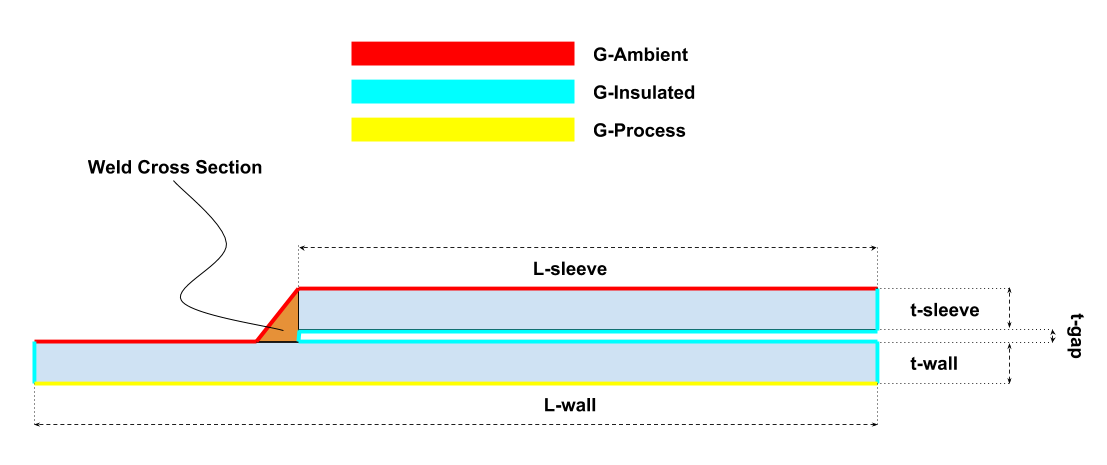
\includegraphics[width=24cm]{img/geometry.png}
}
\caption{Illustration of the axisymmetric sleeve geometry.}
\label{fig:fig1}
\end{sidewaysfigure}